\documentclass[twocolumn]{article}

\usepackage{graphicx}
\usepackage[doi=false,url=false,isbn=false]{biblatex}
\usepackage[spacing, tracking, kerning]{microtype}
\usepackage[top=1in, bottom=1in, left=1in, right=1in]{geometry}
% \newcommand{\subparagraph}{}
\usepackage{titlesec}
\usepackage{float}
\usepackage{color}
\usepackage[usenames,dvipsnames,svgnames,table]{xcolor}
\usepackage{placeins}
% \usepackage{dblfloatfix}
% \usepackage{fixltx2e}
\usepackage[bottom]{footmisc}
% \usepackage{kpfonts}
\usepackage{amsfonts}
\usepackage{relsize}
\usepackage[english]{babel}

\usepackage[colorlinks=false, hidelinks]{hyperref}

\newcommand{\tY}{\checkmark}
\newcommand{\tN}{$\times$}

% \setlength{\columnsep}{4mm}

% \usepackage{caption}
% \usepackage{subcaption}

% \usepackage{fontspec}
% \setmainfont{Humor Sans}

\bibliography{refs}

\graphicspath{{./images/}}

\newcommand{\superscript}[1]{\ensuremath{^{\textrm{#1}}}}

\title{\bfseries\fontsize{20}{1}\selectfont Identifying Compiler Options to Minimize Energy Consumption for Embedded Platforms}
% \author{\fontsize{13}{1}\selectfont
% James Pallister\superscript{\footnotesize1}, Simon Hollis\superscript{\footnotesize2} and Jeremy Bennett\superscript{\footnotesize3} \\[1em]
% 	\fontsize{11}{1}\selectfont\superscript{\footnotesize1} \superscript{\footnotesize2} Department of Computer Science, University of Bristol, \\
% 	\fontsize{11}{1}\selectfont Merchant Venturers Building, Woodland Road, \\
% 	\fontsize{11}{1}\selectfont Bristol, BS8 1UB, United Kingdom. \\
% 	\fontsize{11}{1}\selectfont\superscript{\footnotesize1}\texttt{james.pallister@bristol.ac.uk}
% 	\fontsize{11}{1}\selectfont\superscript{\footnotesize2}\texttt{simon@cs.bris.ac.uk} \\[1em]
% 	\fontsize{11}{1}\selectfont\superscript{\footnotesize3} Palamos House \#104, 66/67 High Street, \\
% 	\fontsize{11}{1}\selectfont Lymington, SO41 9AL, United Kingdom. \\
% 	\fontsize{11}{1}\selectfont \texttt{jeremy.bennett@embecosm.com}
% }

\author{
\parbox{0.33\linewidth}{\centering\fontsize{13}{1}\selectfont James Pallister\\[0.5em]\texttt{jp@cs.bris.ac.uk}}
\parbox{0.33\linewidth}{\centering\fontsize{13}{1}\selectfont Simon Hollis\\[0.5em]\texttt{simon@cs.bris.ac.uk}}
\parbox{0.33\linewidth}{\centering\fontsize{13}{1}\selectfont Jeremy Bennett\\[0.5em]\texttt{jeremy.bennett@embecosm.com}} \\[1.5em]
\parbox{0.66\linewidth}{\centering\fontsize{12}{1}\selectfont
Department of Computer Science, \\
University of Bristol, \\
Merchant Venturers Building, \\
Woodland Road, Bristol, BS8 1UB\\
United Kingdom}
\parbox{0.33\linewidth}{\centering\fontsize{13}{1}\selectfont
Embecosm \\
Palamos House \#104, \\
66/67 High Street, \\
Lymington, SO41 9AL, United Kingdom. \\
}
}
\date{}
\titleformat{\section}{\Large\bfseries\centering\scshape}{}{0em}{}
\titleformat{\subsection}{\normalsize\bfseries}{}{0em}{}

\newcommand{\nsection}[1]{\section{\bfseries #1}}

\newcommand{\todo}[1]{\textbf{\textcolor{red}{#1}}}

% \let\oldcite\cite
% \renewcommand{\cite}[1]{\textsuperscript{\oldcite{#1}}}

\let\oldcaption\caption
\renewcommand{\caption}[1]{\oldcaption{\textup{#1}}}

\begin{document}
\maketitle
\begin{table*}[!hbt]
	\centering
	\begin{tabular}{l l l l l}
		\textbf{Processor} & \textbf{Board name}  & \textbf{RAM} & \textbf{Speed} & \textbf{Extra} \\
		\hline
		ARM Cortex-M0 	 & STM32F0DISCOVERY		& 8KB		& 48 MHz		  & 64KB Flash\\
		ARM Cortex-M3 	 & STM32VLDISCOVERY		& 8KB		& 24 MHz		  & 128KB Flash\\
		ARM Cortex-A8 	 & BeagleBone			& 256MB		& 500 MHz		  & VFP/NEON, superscalar\\
		Adapteva Epiphany 	 & EMEK3				& 32KB/core & 400 MHz		  & FPU, superscalar, 16 core NoC\\
		XMOS L1 		 & XK1					& 64KB		& 100 MHz 		& 4$\times$100MHz hardware threads \\
	\end{tabular}
	\caption{The platforms explored in this paper along with some relevant details.}
	\label{Table:Platforms}
\end{table*}

\section{Abstract}
\raggedbottom
{\bfseries
This paper uses an innovative technique to explore the effect on energy consumption of 87 of the optimizations GCC performs when compiling 10 benchmarks for five different embedded platforms. Hardware power measurements on each platform are taken to ensure all architectural effects on the energy are captured.

A fractional factorial design is used to separate the effects of each optimization and account for interactions between optimizations. We find that in the majority of cases execution time and energy consumption are highly correlated, but the effect a particular optimization may have is non-trivial due to its interactions with other optimizations. Also it is noticed that the structure of the benchmark has a larger effect than the hardware architecture on whether the optimization will be effective, and no one optimization is universally positive for run-time or energy consumption.
}

\section{Introduction}


Energy consumption is rapidly becoming one of the most important design constraints when writing software for embedded platforms. In the hardware space there have been many features such as clock gating to reduce the power consumption of electronic devices. However, inefficient software can negate any gains from the hardware, so the combination of software and hardware must be taken together when exploring energy usage. We focus on embedded platforms, because energy efficiency is particularly important in the design and operation of these processors.

Optimizing for low energy consumption is particularly important for deeply embedded systems, which may have to adhere to a strict power budget. In these systems the processor is only one of the components consuming energy. A previous study characterized the CPU power usage of a mobile phone to be between 10 and 20\% of the total system power\cite{SmartPhonePower}. As the radio consumes roughly 50\% of the power in this system, it can be seen in systems without the GSM component the processor takes a non-trivial proportion of the power.

\begin{figure}[b!]
	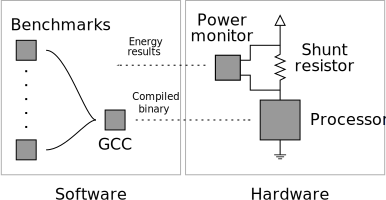
\includegraphics[width=\linewidth]{diagram.pdf}
	\caption{The hardware and software setup used in this paper.}
	\label{Fig:setup}
\end{figure}

Compiler optimizations have the potential for energy savings with no changes to existing applications --- just tweaking the compiler's parameters can have a large effect on the energy consumption. This relationship is complex, with the program, processor architecture and specific compiler options interacting together. Furthermore, different optimization passes interact with each other meaning that an option's efficacy cannot be tested in isolation. For example, inlining a function may mean that more effective common expression elimination can be performed, reducing the instruction count more than either option individually. There have been many approaches attempted to solve this problem using statistical methods\cite{Haneda2005}, genetic algorithms\cite{Lin2008} and iterative compilation\cite{Kisuki1999}. All of these studies conclude that performance can be gained from choosing the correct set of optimizations, but exploring the space to find this set is challenging.

This paper performs an advanced analysis that attempts to separate out the main effect the individual optimizations have from their interactions with other optimizations. These measurements are taken for each optimization grouping, across five platforms and ten benchmarks. We are able to assign an average effect to each optimization, enabling us to see which optimizations significantly affect the energy consumption. Each experiment we perform targets the set of optimizations enabled at a different optimization level, and overall this allows them to be sorted into three categories: decreases energy consumption, has no effect at all, or increases energy consumption.

All the energy measurements in this paper are taken using physical measurement circuitry attached to the processors. This avoids the use of models which could be inaccurate, or modeling synthetic processors with no real world counterpart. A diagram of the software and hardware setup is shown in Figure~\ref{Fig:setup}. By using commonly available platforms and processors along with some more novel architectures, the results are applicable in general while still providing insight into how different types of architectures perform. There are five platforms examined in this paper, shown in Table~\ref{Table:Platforms}.

This paper covers the design and results of the experiments. First, previous work in this space is discussed, along with the novel contribution this paper makes. After this, the approach and a brief discussion of fractional factorial design is listed. Then, the experiments are presented with results. Finally, the results are evaluated and conclusions drawn.


\begin{table}[t]
	\centering
	\begin{tabular}{l c l}
	\textbf{Name}			& \textbf{Source} 	& \textbf{Category} \\
	\hline
	2D FIR					& WCET 		& automotive, consumer	\\
	Blowfish				& MiBench 	& security	\\
	CRC32					& MiBench 	& network, telecomm	\\
	Cubic solver			& MiBench 	& automotive	\\
	Dijkstra				& MiBench 	& network	\\
	FDCT					& WCET 		& consumer	\\
	Float matmult			& WCET 		& automotive, consumer	\\
	Int matmult				& WCET	 	& automotive	\\
	Rjindael				& MiBench 	& security	\\
	SHA						& MiBench 	& network, security	\\
	\end{tabular}
\caption{Benchmarks selected, and the categories they fit into. These are selected from MiBench\cite{MiBench} and the Worst Case Execution Time (WCET)\cite{WCET} suites.}
\label{Table:Benchmarks}
\end{table}

\section{Previous work}

\subsection{Compilers \& Energy}

To date there has been very little work extensively exploring the effect that different compiler optimizations have on energy consumption. However, there have been many studies looking at the effect of optimizations on execution time\cite{Haneda2005}, and several studies suggesting that execution time can be used as a proxy for execution time\cite{CompilingForPerformancePower}.

The topic of performance and energy being highly correlated is addressed in `Is Compiling for Performance == Compiling for Power?'\cite{CompilingForPerformancePower}. The paper explored several different overall optimization levels, as well as four specific optimizations, also using the Wattch simulator to gather energy results. However, the specific optimizations were all applied individually on top of \texttt{-O1}, without exploring any possible interactions between the optimizations. The main conclusion drawn from this study was that most optimizations reduce the number of instructions executed, hence reducing energy consumption and execution time simultaneously.

Of the studies that do look at optimizations and energy, most focus on only a few optimizations in isolation and few consider multiple platforms with different architectural features. Commonly explored optimizations, such as loop unrolling\cite{Ayala2004}, loop fusion\cite{Zhu2004}, function inlining\cite{Kim2012} and instruction scheduling\cite{Toburen1998}, have been examined extensively for different platforms using both simulators and hardware measurements\cite{EffectOfCompilerOptimizationsOnPentium4}.

A drawback of the studies that do explore energy consumption is that many of them choose to use simulators as opposed to taking hardware measurements. The Wattch simulator\cite{Wattch} is commonly used and is designed to allow easy energy measurements while exploring architectural configurations. The accuracy of Wattch is established at being within 10\% of an industry layout-level power tool. Unfortunately, Wattch does not model every hardware component in the processor, which makes it difficult to be certain about the overall energy consumption of the processor.

SimplePower\cite{SimplePower} is another simulator that has been used to explore the effects of the software running on a processor. This simulator targets a five stage RISC pipeline, with models estimating the energy consumption based on the number of transitions on bus signal lines as well as various other components.

Various other models have been created to simulate power consumption of the processor, including complex instruction level models\cite{Steinke2001}, function-level models\cite{Qu2000} and hybrids of the previous two\cite{Blume2007}. These all suffer the drawback that some energy consumption effects may not be modeled, potentially skewing the results.

\subsection{Optimization Choice}

The challenge of choosing the optimizations and their order has been explored and many methodologies proposed for choosing an optimal set of optimizations.

Chakrapani et al attempt to classify optimizations by the effect they have on performance and energy\cite{WhatCanAPoorCompilerDo}. This paper took both hardware measurements and used a gate-level simulation to derive the results, separating the optimizations into three classes:
\begin{itemize}
	\setlength{\itemsep}{0em}
	\vspace{-1mm}
	\item Reduction in energy consumption due to increase in performance. These optimizations reduce the number of cycles or instructions needed to complete the application and thus less overall work is done.
	\item Optimizations that reduce energy while not improving the performance. Scheduling instructions to reduce switching often falls into this category.
	\item Optimizations that increase energy consumption or performance.
\end{itemize}

Iterative compilation has been examined as a possibility for choosing optimizations that reduce power by Gheorghita et al\cite{IterativeCompilationForEnergy}. In this paper, the effect of different loop unrolling and loop tiling parameters on energy consumption is examined for three linear-algebra-based benchmarks using a simulator. The paper concluded that iterative compilation was an effective method of decreasing energy consumption as well as improving performance.

Other approaches have looked at genetic algorithms for optimization selection\cite{Lin2008} and optimization phase ordering\cite{Almagor2004}. While these techniques are shown to be effective, they have the drawback that the reasons behind the optimization's select is non-obvious.

These techniques do not expose the relationships between optimizations, instead opting to search though the optimization space and make a best guess where to look next. In this paper, we improve these shortcomings using a technique called fractional factorial designs\cite{BoxHunter} to explore the most effective options and the interactions between them.

Fractional factorial design, as a method for exploring the interactions of compiler optimizations was explored in the paper `Feedback-Directed Selection and Characterization of Compiler Optimizations'\cite{IntelPaper}. Nine optimizations were examined, using a fractional factorial technique to isolate the interactions and choose a set of optimizations that gave better performance than just enabling all the optimizations.

A similar study conducted by Patyk et al\cite{EnergyReductionCompilerOptions}, extended this work to energy efficiency. The study explored a range of GCC's options, with an aim to reduce energy consumption by identifying significant optimizations then excluding them from further exploration, using fractional factorial designs. We use this technique to analyse the optimizations rather than optimize for the energy consumption.

These methods of testing over many different compilations is a significant overhead when finding an optimal set. The MILEPOST GCC\cite{Fursin2011} study implemented one alternative to this by using machine learning to guess which optimization flags would best apply to a given program. Features are extracted from the program, which are then matched against previous known results from previous compilations. This allows a set of optimizations to be estimated from just the source code.

\subsection{Optimizations Targeting Energy}

The previous studies all look at how to utilize existing optimization to target energy consumption. However, all of these optimizations were written with the aim of reducing execution time, not energy consumption. Several other techniques have been proposed to develop optimizations that specific target energy consumption.

An analysis of the techniques the compiler can perform to optimize for energy was carried out by Tiwari, Malik and Wolfe\cite{CompilationTechniquesForLowEnergy}. They identified several possible techniques that compilers could use to reduce the energy consumption of programs:
\begin{itemize}
	\setlength{\itemsep}{-0.4em}
	\vspace{-2mm}

	\item Reorder instructions to reduce switching.
	\item Reduce switching on address lines.
	\item Reduce memory accesses.
	\item Improve cache hits.
	\item Improve page hits.
\end{itemize}

It is expected that optimizations covering some of these points will have an effect on energy. The last three will also normally increase performance as well as reduce energy.

Several novel types of compiler optimizations have been proposed. Seth et al\cite{Seth2001} explored the possibility of using the compiler to insert \texttt{idle} instructions automatically, increasing the execution time up to a set limit. Using the SIMD pipeline has been shown to decrease energy consumption\cite{Ibrahim2009} by roughly 25\%. Scheduling instructions to minimize the inter-instruction energy cost was evaluated to be another effective method to reduce a programs energy consumption\cite{Parikh}.

\section{Approach}

The majority of the studies listed previously only examine one platform, and it is currently unknown whether the results would apply across several different platforms. Furthermore, the iterative compilation and other adaptive techniques used can leave holes of potential combinations of optimizations unexplored (due to the huge numbers of combinations possible). This lead to the most optimal configurations not being found. In this paper we present another technique for testing the effectiveness of large numbers of compiler optimization flags and their impact on energy consumption and run-times. The technique is based on the concept of fractional factorial designs (discussed in a following section).

To explore the impact of the optimizations, a realistic set of test input programs is needed. Since there have been many attempts to find representative programs, but none apply to a wide range of embedded processing systems, a set of benchmarks has been derived from contemporary suites. This set of 10 benchmarks (shown in Table~\ref{Table:Benchmarks}) covers real world and synthetic applications across different aspects of the target platform. Previous work on modeling the energy consumption of processors has shown that the pipelines and functional units enabled have a significant impact on the energy consumption. To cover these points, the benchmarks were chosen to cover the following coarse criteria:
\begin{itemize}
	\setlength{\itemsep}{0em}
	% \setlength{\parskip}{1pt}
	\vspace{-1mm}
	\item \textbf{Integer pipeline intensity.} The frequency at which integer arithmetic instructions occur.
	\item \textbf{Floating point intensity.} The frequency of floating point operations.
	\item \textbf{Memory intensity.} Whether the program requires a large amount of memory bandwidth or not.
	\item \textbf{Branch frequency.} How often the code branches.
\end{itemize}

Similar categories of instruction types have been used previously to give a high level overview of the type of computation an application is performing\cite{Hennessy2012}. MiBench\cite{MiBench} uses a finer-grained version of these categories in its analysis.

These benchmarks were constructed to run on the `bare metal' --- no host OS needed. This prevents the benchmark from being preempted by an operating system performing a background task and reducing the accuracy of the results. The benchmarks must also be chosen carefully with regards to cache performance. In this study we bypassed the issue entirely by choosing benchmarks that were small enough to fit into the L1 cache of the only platform with caches (Cortex-A8). All the measurements were `warm-start', minimizing the impact on the results that the cache would have.

In this paper we explore the impact of compiler optimizations using the GCC toolchain on the architectures in Table~\ref{Table:Platforms}. GCC exposes its various optimizations via a number of flags that can be passed to the compiler. We explore what flags are and are not significant for energy consumption and execution time.

The experiments are performed with different benchmarks, so a full picture of architecture, optimization and application can be seen. By taking this combination of all three items, the following points of interest can be explored:
\begin{itemize}
	\setlength{\itemsep}{0em}
	\vspace{-1mm}
 	\item The relationship between time and energy.
 	\item Architectural and application effects.
 \end{itemize}

\section{Hardware Setup}

All the measurements were taken using the INA219 power monitoring IC\cite{INA219}, which provides power, current and voltage outputs.

The Cortex-M0 and Cortex-M3 boards both have a single measurement point, recording the power consumed by the whole microprocessor. For the BeagleBone there are three available measurement points: the Cortex-A8 core (including caches), on-chip peripherals (power management, bus controllers) and the external SDRAM memory IC. This allows the effect of the compiler optimizations on the memory to be recorded. Adapteva's Epiphany board has two measurement points: the core power consumption and IO power consumption, whereas the XMOS board's measurement point gathers power consumption data for the core of the processor.

\section{Fractional Factorial Design}

\begin{figure}[bt]
	\centering
	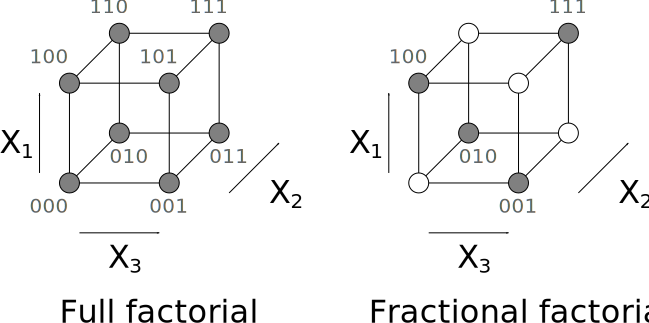
\includegraphics[width=0.9\linewidth]{ffd.pdf}
	\caption{Reducing a 3-factor full factorial design to a `half fraction' design.}
	\label{Fig:FFDTut}
\end{figure}

GCC has over 150 different options that can be enabled to control optimizations. The majority of these options are binary --- the optimization pass is either enabled or disabled. To further complicate matters, an optimization path may be affected by other passes happening before it. As it is infeasible to test all possible combinations of options, a trade-off has to be made. One of our main contributions is to deploy fractional factorial design (FFD) to massively reduce the exploration space, whilst still identifying the options that contribute to run-time and energy. This approach has been explored before in `Feedback-Directed Selection and Characterization of Compiler Optimizations'\cite{IntelPaper}, where nine optimizations were explored in just 35 tests as opposed to the 512 required for a full factorial design.

An example \textit{full} factorial design is shown on the left of Figure~\ref{Fig:FFDTut}. This example shows three two-level factors with every possible combination enumerated. A fractional factorial design with the number of tests halved is shown on the right.

The drawback to this approach is that the high-order interactions (effects due to multiple options being enabled) between options will not be discernible. Fortunately this is not usually a problem as these types of interactions are statistically rare. The degree to which this happens is specified by the FFD's resolution. A resolution 5 design ensures that the main effects are not aliased with anything lower than 4th order interactions.

Using the Yates algorithm\cite{BoxHunter} the effect for any single or combination of factors can be found from the data. This gives an average estimation for how much this factor or interaction affects the result of the experiment. The Mann-Whitney statistical test is used to determine whether the factor represents a significant change in performance as detailed in \cite{EnergyReductionCompilerOptions} and \cite{Haneda2005}.


\begin{figure}[t!]
	\includegraphics[width=\linewidth,clip,trim=0.5cm 0 2cm 1.8cm]{cortex-m0/O1_main_effects_blowfish.pdf}
	\caption{Blowfish benchmark on the Cortex-M0 platform. Individual options enabled at \texttt{O1} are listed.}
	\label{Fig:BlowfishMainEffects}
\end{figure}

\begin{figure}[t!]
	\includegraphics[width=\linewidth,clip,trim=0.5cm 0 2cm 1.8cm]{cortex-m3/O2_main_effects_fdct.pdf}
	\caption{FDCT benchmark on the Cortex-M3 platform. Individual options enabled at \texttt{O2} are listed.}
	\label{Fig:FdctO2MainEffects}
\end{figure}


All FFDs used were generated by R\cite{R}, using the FrF2 library\cite{FrF2}.

\section{Results}

\subsection*{Time and Energy}


\begin{figure*}[tb!]
	\centering
	\includegraphics[width=\textwidth,clip, trim=0cm 0cm 0 2.1cm]{levels.pdf}
	\caption{Energy, time and power results for benchmark-platform combinations. Optimization levels \texttt{O0} to \texttt{O4}. \texttt{O4} is \texttt{O3} with link-time optimization. The last point is \texttt{Os} --- optimize for space. }
	\label{Fig:OverallView}
\end{figure*}
This study aims to establish whether execution time and energy consumption are highly correlated in the majority of cases. This hypothesis underlies many of the assumptions of the energy-efficiency community relating to the best way forward in producing energy-efficient software. Overall it was found that this hypothesis is correct, with some small divergences for the Cortex-A8. This section presents the results supporting this conclusion, and discusses some of the cases where there is a difference between energy consumption and execution time.

A high level overview of each platform and benchmark for different optimization levels is given in Figure~\ref{Fig:OverallView}. This figure shows a small line graph for each combination, displaying the effect of the broad optimization levels \texttt{O1}, \texttt{O2}, \texttt{O3}, \texttt{O4} (\texttt{O3} with link time optimization) and \texttt{Os} (optimize for space) on time, energy and power. The following section discusses the conclusions that can be drawn from this graph.

Further results showing the correlation between time and energy are shown in Figure~\ref{Fig:BlowfishMainEffects}. This shows the main effect each optimization has on the runtime and energy consumption, as calculated by the FFD. As these results come from a total of 2048 seperate runs, even a small percentage change is statistically significant. This significance is calculated using the Mann-Whitney test --- the bracket above the bars indicates when the results satisfies the following hypothesis: it is 95\% certain that the result represents a signficant impact on the energy consumption of the benchmark.

Figure~\ref{Fig:FdctO2MainEffects} highlights a discrepancy that occurred between execution time and energy consumption, even for very similar optimizations. The first two options listed (\texttt{-fschedule-insns} and \texttt{-fschedule-insns2}) both schedule instructions to reduce pipeline stalls. However the latter option performs its scheduling pass after register allocation, where as the first performs it before. In this case scheduling before the register allocation reduces the energy consumption by much more than the execution time.

\subsection{Architectures and their Effects}

The following paragraphs explore the architectural details of the processors, and how they are connected to the energy consumption.

For the Cortex-M0, very little difference between energy and time is seen due to it being the simplest processor tested: it has a three stage pipeline without forwarding logic. The pipeline never stalls unless it encounters a load or a branch, in which case it always stalls. The Cortex-M3 exhibits very similar behavior, with some very slight differences between energy and time. The micro-architecture in this processor is more complex, featuring branch speculation and a larger instruction set\cite{Yiu2010}.

The XMOS processor has a four stage pipeline, similar to the Cortex-M3 in complexity and performance. It should also be noted that the compiler for the XMOS processor uses an LLVM backend for code generation, featuring different optimizations. Due to this the result set for this processor is not as extensive as the other four.


The Epiphany processor also sees a large correlation between the energy consumption and execution time. There is some divergence for a few of the benchmarks. These are likely when the superscalar core in the processor has been able to dispatch multiple instructions simultaneously.

The greatest difference between energy and time was discovered while using the Cortex-A8. For the majority of the benchmarks the execution time reduces more than the energy. This is due to multiple instructions being executed simultaneously by the core, reducing the amount of time taken but not the energy consumption, as the same total work is still being done. The gap is also seen to widen at the \texttt{O2} level, due to instruction scheduling being enabled there.


\subsection{Efficient SIMD Units}

\begin{figure}[t!]
	\includegraphics[width=\linewidth,clip,trim=0.5cm 0 2cm 1.8cm]{cortex-a8/O3_main_effects_2dfir.pdf}
	\caption{2D FIR benchmark on the Cortex-A8 platform. Individual options enabled at \texttt{O3} are listed.}
	\label{Fig:O3_2dfir_A8}
\end{figure}


\begin{table}
	\centering
	\begin{tabular}{c p{0.3\linewidth} p{0.4\linewidth}}
		\bfseries NEON & \bfseries Instruction Dependencies & \bfseries Continuous Power Consumption \\
		\hline
		No & \centering Yes & {\hspace{0.85cm} 168000 uW } \\
		No & \centering No & {\hspace{0.85cm} 195000 uW } \\
		Yes & \centering Yes & {\hspace{0.85cm} 158000 uW } \\
		Yes & \centering No & {\hspace{0.85cm} 159000 uW } \\
	\end{tabular}
	\caption{Micro-benchmark results for multiplications on the NEON unit, with and without inter-instruction dependencies.}
	\label{Table:SIMD}
\end{table}

An interesting effect is seen in 2D FIR for the Cortex-A8. The execution time decreases more than the energy consumption up to \texttt{O2}, but when enabling \texttt{O3} the energy decreases more than the execution time. On further investigation, this is caused bt the \texttt{-ftree-vectorize} optimization having an impact on energy consumption with no change in execution time (shown in Figure~\ref{Fig:O3_2dfir_A8}). This option vectorizes loops, so that SIMD instructions can be inserted.

Further investigation of the NEON SIMD unit was done using some small micro-benchmarks. The results of these are shown in Table~\ref{Table:SIMD}, showing for multiplication the NEON unit uses a lot less power than using the normal Cortex-A8 multiplier. This shows that by using the hardware to its full capacity, the greatest energy savings can be achieved.

% talk about what the results are briefly
% second and third order interactions

\begin{table*}
	\centering
	\begin{tabular}{l >{\ttfamily} c >{\ttfamily} c >{\ttfamily} c >{\ttfamily} c }
		\bfseries Benchmark&\rmfamily\bfseries Cortex-M0&\rmfamily\bfseries Cortex-M3 & \rmfamily\bfseries Cortex-A8		& \rmfamily\bfseries Epiphany\\
		\hline
		2dfir          &  E        &  T, G, I  &  N, G, B  &  I, A, D  \\
		blowfish       &  C, J, E  &  J, C, G  &  K, C, E  &  D, P, I  \\
		crc32          &  F        &  F        &  F, G     &  None     \\
		cubic          &  A, H     &  A, H     &  A        &  A, H, R  \\
		dijkstra       &  H, A, C  &  F, H, A  &  F, H, A  &  H, A     \\
		fdct           &  J, G, D  &  J, G, K  &  M, K, J  &  A, I, D  \\
		float\_matmult &  B, E     &  B, E, G  &  N, L     &  D, I, A  \\
		int\_matmult   &  B, E, C  &  B, L, F  &  L, N, M  &  A, I, D  \\
		rijndael       &  C, B, O  &  C, B, O  &  K, C, S  &  D, K, B  \\
		sha            &  C, B, E  &  B, C, F  &  B, C, M  &  D, B, Q  \\

	\end{tabular} \\[1em]

	\begin{tabular}{>{\fontsize{9}{1}\selectfont}c | r >{\ttfamily\fontsize{9}{1}\selectfont}l
					% >{\fontsize{8}{1}\selectfont}c | r >{\ttfamily\fontsize{8}{1}\selectfont}l
					>{\fontsize{9}{1}\selectfont}c | r >{\ttfamily\fontsize{9}{1}\selectfont}l }
	\bfseries ID & \multicolumn{2}{l}{\bfseries Count\hspace{1.2cm}Flag} &\bfseries ID & \multicolumn{2}{l}{\bfseries  Count\hspace{1.2cm}Flag} \\
	\hline
	\fontsize{9}{1}\selectfont
	A & 12 & -ftree-dominator-opts & 	 K & 5  & -fschedule-insns \\
	B & 12 & -ftree-loop-optimize &      L & 3  & -finline-small-functions \\
	C & 11 & -fomit-frame-pointer &      M & 3  & -fschedule-insns2 \\
	D & 8  & -fdce &                     N & 3  & -ftree-pre \\
	E & 7  & -fguess-branch-probability& O & 2  & -ftree-sra \\
	F & 7  & -fmove-loop-invariants &    P & 1  & -fipa-profile \\
	G & 7  & -ftree-ter &                Q & 1  & -ftree-pta \\
	H & 7  & -ftree-fre &                R & 1  & -fcombine-stack-adjustments \\
	I & 6  & -ftree-ch &                 S & 1  & -fgcse  \\
	J & 5  & -ftree-forwprop &           T & 1  & -fpeephole2 \\
	\end{tabular}


	\caption{Table showing the most effective option for each platform-benchmark combination. Options considered were
	optimizations enabled by \texttt{O1}, \texttt{O2} and \texttt{O3} levels.}
	\label{Table:BestFlags}
\end{table*}


\subsection{The Universality of Flags}

An interesting problem for compiler designers is how to choose an optimal set of flags across different hardware platforms and applications. This section explores which individual flags had the largest effect in our experiments and establishes whether a set of consistently good optimizations are seen across each benchmark and platform. Table~\ref{Table:BestFlags} lists the results for this section, with the top three optimization flags (where that optimization has a significant effect, as per the Mann-Whitney test) identified for each benchmark and platform combination.  Each letter represents an optimization that is labeled in the the table below. This table also specifies the number of times this flag occurs.

Only 20 out of 82 options examined (the number of flags enabled by \texttt{O1}, \texttt{O2} and \texttt{O3}) appear in the table. This adds weight to the argument that many of the options have little effect on the energy consumption (and performance).

It can be seen that for the ARM platforms a similar set of options appears for the same benchmarks. Common options for the same benchmarks are expected, as optimizations are triggered by the structure of the source code. However, the opposite of this is seen for the Epiphany platform --- there are three optimizations that are consistently effective at reducing energy consumption. In particular, an unusual option to be consistently effective is \texttt{-fdce}. This optimization is dead code elimination, eliminating code which is never used by the application. However, this can allow the compiler to eliminate parts of the control flow graph, removing branches and decreasing the overall amount of work the application performs.

The optimization listed most frequently in the table is \texttt{-ftree-dominator-opts}. The prevalence of this flag is likely due to it enabling several simple optimization passes, performing optimizations such as copy propagation and expression simplification. Another effective optimization is \texttt{-fomit-frame-pointer}. This optimization frees an additional register for general use by not using a frame pointer. This optimization is seen frequently on the ARM platforms, however not at all on the Epiphany. This is likely due to the ARM processors suffering from greater register pressure as they only have 16 registers compared to the Epiphany's 64.

\begin{figure*}[t!h]
	\includegraphics[width=\linewidth,clip,trim=0.5cm 1.0cm 0cm 1.8cm]{cortex-m3/O1_addsub_blowfish.pdf}
	\caption{Blowfish benchmark on the Cortex-M3 platform. Individual options are enabled or disabled on top of the \texttt{O1} optimization level.}
	\label{Fig:AddsubO1Blowfish}
\end{figure*}


We see some interesting correlations between platforms. The optimizer has trouble optimizing the crc32 benchmark, with the Cortex-M0 and Cortex-M3 only having one optimization which has any significant effects (\texttt{-fmove-loop-invariants}). The Cortex-A8 sees an additional optimization having an effect, however this is still secondary to the previously mentioned optimization (it had an average of a 1.3\% effect on the energy consumption).

As observed in previously, similar options are seen to affect the energy consumption across benchmarks. This is due to the optimizations being targeted to specific high level language constructs, which only appear in some of the benchmarks. These results show the difficulty of choosing one optimization which is good in all cases. In many cases the instruction set and micro-architecture of the processor have a large effect on how much the energy consumption is reduced, meaning that a singularly good optimization cannot be chosen.

\subsection{Optimization Chaos}

The previous section concluded that there was not a single optimization that was universally good for all benchmarks and platforms. In this section, this is extended further, concluding that there is a very chaotic relationship between the platform, benchmark, optimization and the effectiveness of the optimization.

Examining the correlation between optimizations and their effects is a complex issue. Due to non-linear interactions, one would expect that the prediction of effects is difficult. This is borne out by our experimental results: as seen in previous figures~\ref{Fig:BlowfishMainEffects} and~\ref{Fig:FdctO2MainEffects}, less than a third of the options have a significant impact. For the other optimizations, higher order interactions cause unpredictable effects, where enabling or disabling a particular optimization can completely change the effect of many other subsequent optimization passes.

In Figure~\ref{Fig:AddsubO1Blowfish}, several unexpected effects worthy of further investigation can be seen. This graph shows individual optimizations being turned on and off, using the \texttt{O1} optimization level as a base. The flags on the left of the \texttt{O1} section were found to decrease the energy consumption when disabled, an effect not seen in the FFD results. These flags were chosen for further exploration.



To explore the inconsistency, a small case study was performed, where all combinations of four options were explored. The energy figures for exhaustive exploration can be seen in Table~\ref{Table:Exhaustive}, with the aim being to ascertain whether the effect of this energy reduction would compound with multiple flags. The \texttt{O1} column of this table shows the results of the options applied over the \texttt{O1} optimization level. The \texttt{O2} column shows the same but on top of the \texttt{O2} optimization level.

From the \texttt{O1} column this it can be seen that there are many interactions occurring between the options, as simply turning all of these options off does not decrease the energy (in fact it increases the consumption by 1.81\%). Furthermore, when disabled individually, \texttt{-fguess-branch-probability} and \texttt{-ftree-dominator-opts} decrease the energy by 2.49\% and 1.76\% respectively. However when both enabled, the energy consumption (relative to \texttt{O1}) is only 0.93\% less --- worse than each flag individually.

\begin{table}[thb]
	\centering
	\begin{tabular}{c <{\hspace{-2mm}} c <{\hspace{-2mm}} c <{\hspace{-2mm}} c <{\hspace{-2mm}} c r@{.}l c r@{.}l }
		& & & \multicolumn{3}{c}{\null\hfill\bfseries \texttt{O1}} & \multicolumn{3}{c}{\hfill\bfseries \texttt{O2}} \\
		\bfseries X1 & \bfseries X2 & \bfseries X3 & \bfseries X4 & \bfseries (mJ) 	 & \multicolumn{2}{c}{\bfseries (\%)} &
		\bfseries (mJ) 	 & \multicolumn{2}{c}{\bfseries (\%)} \\
		\hline
		\tY&\tY&\tY&\tY& 5780 & 0&00 	&  5480 &  0&00\\
		\tN&\tY&\tY&\tY& 5640 & -2&49 	&  5540 &  1&00\\
		\tY&\tN&\tY&\tY& 5680 & -1&76 	&  5480 & -0&05\\
		\tN&\tN&\tY&\tY& 5730 & -0&93 	&  5620 &  2&49\\
		\tY&\tY&\tN&\tY& 5650 & -2&28 	&  5490 &  0&09\\
		\tN&\tY&\tN&\tY& 5720 & -0&97 	&  5580 &  1&75\\
		\tY&\tN&\tN&\tY& 5610 & -2&90 	&  5480 &  -0&03\\
		\tN&\tN&\tN&\tY& 5640 & -2&33 	&  5530 &  0&85\\

		\tY&\tY&\tY&\tN& 5760 & -0&34 	&  5460 &  -0&43\\
		\tN&\tY&\tY&\tN& 5720 & -1&09 	&  5480 &  0&03\\
		\tY&\tN&\tY&\tN& 5860 & 1&45 	&  5490 &  0&15\\
		\tN&\tN&\tY&\tN& 5960 & 3&08 	&  5480 &  0&00\\
		\tY&\tY&\tN&\tN& 5890 & 1&91 	&  5470 &  -0&19\\
		\tN&\tY&\tN&\tN& 5870 & 1&61 	&  5570 &  1&57\\
		\tY&\tN&\tN&\tN& 5690 & -1&56 	&  5480 &  -0&03\\
		\tN&\tN&\tN&\tN& 5880 & 1&81 	&  5510 &  0&41\\
	\end{tabular}\\[1em]
	\caption{Exhaustively exploring 4 options compared to \texttt{O1} and \texttt{O2}. (Cortex-M3 with blowfish benchmark). Legend in Table~\ref{Table:ExhaustiveLegend}.}
	\label{Table:Exhaustive}
\end{table}
\begin{table}[thb]
	\centering
	\begin{tabular}{l p{0.65\linewidth}}
		\bfseries Key & \bfseries Option \\
		\hline
		X1 & \texttt{-fguess-branch-probability}  \\
		X2 & \texttt{-ftree-dominator-opts}  \\
		X3 & \texttt{-ftree-ch} \\
		X4 & \texttt{-fif-conversion} \\
		Abs (mJ) & Absolute energy measurement in millijoules. \\
		\texttt{O1} (\%) & Percentage relative to \texttt{O1}. \\
		\texttt{O2} (\%) & Percentage relative to \texttt{O2}. \\
	\end{tabular}
	\caption{Legend for Table~\ref{Table:Exhaustive}.}
	\label{Table:ExhaustiveLegend}
\end{table}


Different results are seen entirely in the \texttt{O2} column, with options that decreased energy consumption on top of \texttt{O1} have little or the opposite effect when applied on top of \texttt{O2}.

This unpredictability suggests that these options have many interdependencies that are difficult to predict upfront. It also makes choosing an optimal set of optimizations very challenging. Therefore, one of our findings is that it is very unlikely any accurate prediction mechanism for considering an optimization and its effect on a target system exists. The effect will always be highly dependent on the application to be used and the platform upon which it resides.

\section{Modeling}

As mentioned earlier, it is unlikely that a model exists that can predict how a set of optimizations will perform. However, if one were to be found, it would allow designers to make fast guesses about how their program will be optimized.

Given our previous conclusions regarding the difficulty of correlating optimizations against improvements, we would expect such a model to yield only mediocre results. To explore this assertion we attempted to create such a model. Our method was to construct a linear model using the data from the FFD. The resulting model fails to capture the higher order effects of some of the benchmarks. Figure~\ref{Fig:twoway_cubic} shows the cubic benchmark on the Cortex-M0 along with prediction, when pairs of optimizations are turned on.

The three options with the highest impact are the same in both model and actual results, but the order is different. The interactions between these options are also slightly different in the model. While the model still identifies the most significant factors, the chaotic pattern seen in the actual results is not captured by this model.


\begin{figure*}
	\centering
    \begin{minipage}[l]{0.98\columnwidth}
        \centering
		\includegraphics[width=1.0\linewidth, clip, trim= 8.8cm 0 4.8cm 2cm]{cortex-m0/o1cub_-7p5_10.png}
    \end{minipage}
    \hfill
    \begin{minipage}[l]{0.07\columnwidth}
        \centering
        \includegraphics[width=1.0\linewidth, clip, trim= 29.1cm 0 0cm 1.7cm]{cortex-m0/o1cub_-7p5_10.png}
    \end{minipage}
    \hfill
    \begin{minipage}[r]{0.95\columnwidth}
        \centering
		\includegraphics[width=0.9\linewidth, clip, trim= 8.8cm 0 7cm 2cm]{cortex-m0/o1cub_-7p5_10_pred.png}
    \end{minipage}
    \caption{Effect on execution time and energy consumption from turning on just two optimization flags at a time (all other options off). The actual result is shown on the left, and the prediction on the right. The analysis used the cubic benchmark on the Cortex-M0.}
    \label{Fig:twoway_cubic}
\end{figure*}



\section{Discussion}

In this section, we explore any sources of error in our measurements and corresponding conclusions.
Using the FFD method allows a good estimate of the impact each compiler option has, while accounting for possible interactions between the options.

The hardware measurements have several sources of error. The most apparent errors are variations in the timing: the INA219 is polled at intervals of roughly 1~ms and the power measurement integrated over this. The interval is occasionally larger - the bottleneck was transferring the data over the communication link back to the PC. The ADC in the INA219 also fluctuated by $\pm$30~$\mu$V, however this was close to the noise floor of the measurements, so had no significant effect on the results.

\section{What does this mean for the compiler writer?}

The existing collections of optimizations at the various levels (\texttt{O1}, etc.) do a good job of optimizing for performance, and consequently, energy. These strike a good balance between ease of use and performance. However, they will never be as optimal as searching through the full optimization space. To avoid running many tests to find a good solution, developing machine-learning compiler technologies similar to MILEPOST GCC would be fitting. A reasonable set of optimizations could be predicted, greatly reducing time spent searching. This is especially true as the effectiveness and types of optimizations was found to be heavily based on the structure of the application being compiled itself. Implementing this would reduce compile times as well as the energy and execution time of the application.

This study focused on GCC, as it is a mature compiler supporting many different platforms and optimizations. As an alternative, the LLVM compiler\cite{LLVM} is relatively new, but has a well defined set of optimization passes, whose order can easily be specified. This extra flexibility means there may be a better solution to find, but also that it is essentially searching for a sharper needle in a bigger haystack. The benefits from having this much larger space to explore may not be worth the trade-off of the time it takes to find it. Therefore, it is unlikely that we will ever be able to obtain the goal of easy optimization for run-time or energy, and will remain constrained to sub-optimal but balanced sets of flags such as \texttt{O3} or longer search-based methods.

\section{Conclusion}

In this study, we used fractional factorial design to explore the execution time and energy consumption optimization space for compilers. We observed its effect on energy consumption and draw conclusions about what optimizations can and cannot provide global improvements in performance. In comparison to other methods such as iterative compilation, FFD is a good alternative because with a small number of runs the options affecting the energy consumption can be quickly found.

We have shown that the assumption of no higher order compiler optimization interactions is incorrect. We substantiate this by showing the amount of variation seen between tests with different options enabled. In general, exploring the optimization space is time intensive and difficult to explore in a structured manner. Therefore, FFD and iterative techniques will always be necessary.

We have shown that in almost all cases the execution time and energy consumption of a benchmark are highly correlated, across five different platforms. Most of the current optimizations in GCC reduce the total workload of the program, which in turn reduces both the time and the energy. This could be an artifact of all current optimization passes being designed to increase performance: energy reduction is purely a side-effect. If energy reduction without a corresponding change in performance is required, other optimizations will have to be implemented.

It is very difficult to predict which optimizations will have an effect, whether that effect is positive, negative, or not impacting the benchmark at all. Among the options that do have an effect, there are many interactions. This results in a very chaotic space to explore, that empirically is affected more by the choice of benchmark than the platform it is running on. This highlights the importance of using more than one benchmark, and having that set of benchmarks cover different types of applications. In practical use, this means that no benchmark can be said to have similar optimizations to any related program, and the need for program-specific optimization will always exist.

\printbibliography

\end{document}
